% Author: Marek Fiser <tikz at marekfiser.cz>
% MESIF protocol: http://en.wikipedia.org/wiki/MESIF_protocol
\documentclass[tikz, border=10pt]{standalone}
%%%<
\usepackage{verbatim}
%%%>
\begin{comment}
:Title: MESIF protocol
:Tags: Diagrams;Block diagrams;Computer science
:Author: Marek Fiser
:Slug: mesif

A diagram describing the MESIF protocol: http://en.wikipedia.org/wiki/MESIF_protocol
\end{comment}
\usetikzlibrary{arrows}
\begin{document}
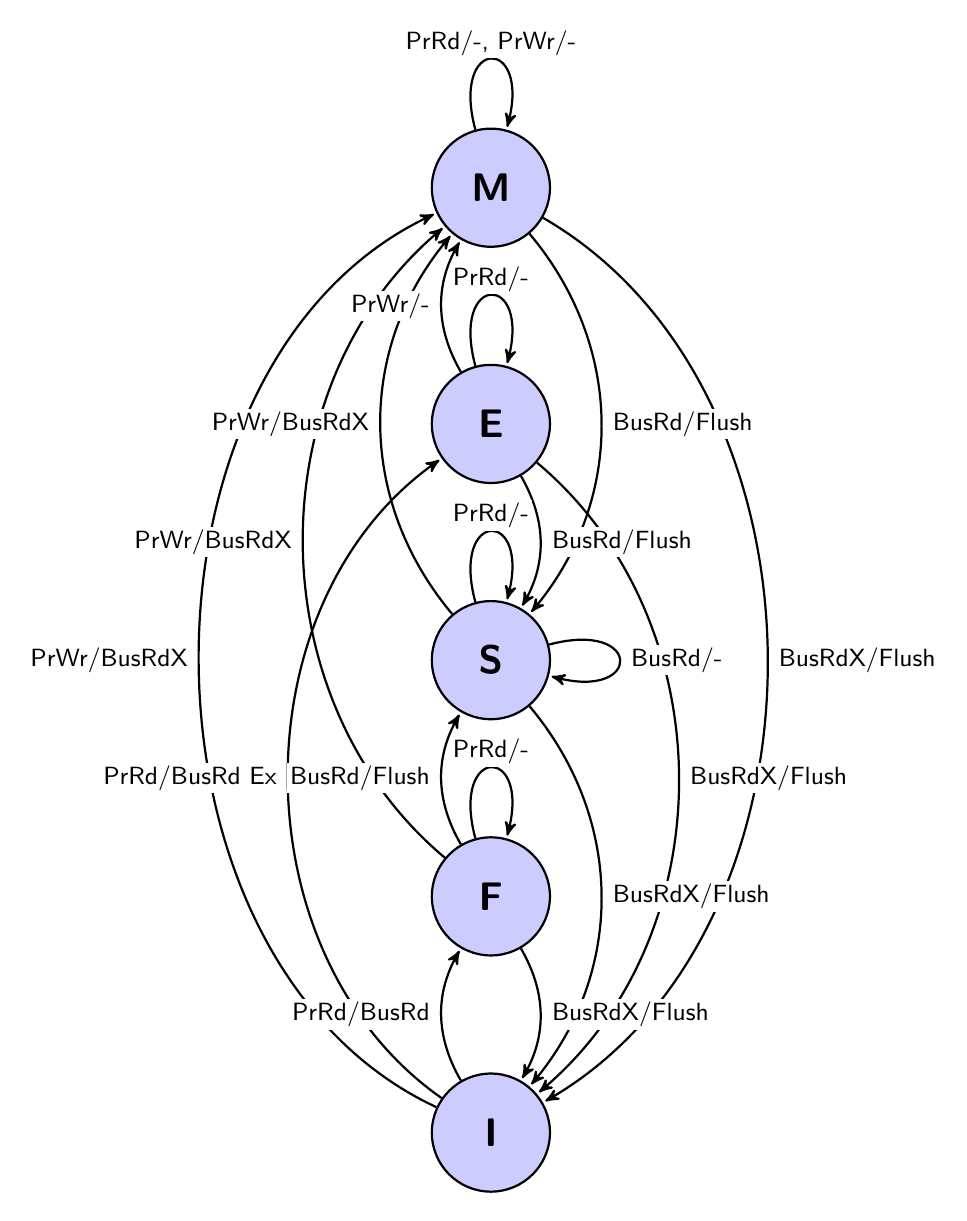
\begin{tikzpicture}[->,>=stealth',shorten >=1pt,auto,node distance=3cm,
  thick,main node/.style={circle,fill=blue!20,draw,
  font=\sffamily\Large\bfseries,minimum size=15mm}]

  \node[main node] (M) {M};
  \node[main node] (E) [below of=M] {E};
  \node[main node] (S) [below of=E] {S};
  \node[main node] (F) [below of=S] {F};
  \node[main node] (I) [below of=F] {I};

  \path[every node/.style={font=\sffamily\small,
  		fill=white,inner sep=1pt}]
  	% Right-hand-side arrows rendered from top to bottom to
  	% achieve proper rendering of labels over arrows.
    (M) edge [loop above] node {PrRd/-, PrWr/-} (M)
        edge [bend left=60] node[right=1mm] {BusRdX/Flush} (I)
        edge [bend left=40] node[right=1mm] {BusRd/Flush} (S)
    (E) edge [loop above] node {PrRd/-} (E)
        edge [bend left=50] node[right=1mm] {BusRdX/Flush} (I)
        edge [bend left=30] node[right=1mm] {BusRd/Flush} (S)
    (S) edge [loop above] node {PrRd/-} (S)
        edge [loop right] node[right=1mm]  {BusRd/-} (S)
        edge [bend left=40] node[right=1mm] {BusRdX/Flush} (I)
    (F) edge [bend left=30] node[right=1mm] {BusRdX/Flush} (I)
        
  	% Left-hand-side arrows rendered from bottom to top to
  	% achieve proper rendering of labels over arrows.
    (I) edge [bend left=65] node[left=1mm] {PrWr/BusRdX} (M)
        edge [bend left=55] node[left=1mm] {PrRd/BusRd Ex} (E)
        edge [bend left=30] node[left=1mm] {PrRd/BusRd} (F)
    (F) edge [loop above] node {PrRd/-} (F)
        edge [bend left=50] node[left=1mm] {PrWr/BusRdX} (M)
        edge [bend left=30] node[left=1mm] {BusRd/Flush} (S)
    (S) edge [bend left=40] node[left=1mm] {PrWr/BusRdX} (M)
    (E) edge [bend left=30] node[left=1mm] {PrWr/-} (M);
\end{tikzpicture}
\end{document}
